\section{Experiments} \label{sec:exp}
We evaluate our theoretical findings and our proposed criterion. We anticipate that the value of data is significantly affected by misspecification, so that labeled data offers an insignificant value versus unlabeled (i.e., a small value ratio) for a well-specified model, but becomes more valuable as the misspecification level increases. We hypothesize that combining both labeled and unlabeled data can offer a superior estimate (as compared to relying one or the other alone). Finally, we expect that the bias due to misspecification is reflected downstream for a variety of models. 

\subsection{Synthetic Data}

Our first class of experiments use synthetic data to validate three principles:
\begin{itemize}
    \item Learning from unlabeled data incurs an additional bias due to misspecification, which can be mitigated by using medians under certain conditions on $m$ and $d$.
    
    \item The data value ratio is roughly constant and small for a well-specified model, and scales with misspecification.
    
    \item 
\end{itemize}

\paragraph{Correcting for misspecification} For a reasonable synthetic data distribution, we 

\paragraph{Choosing between labeled and unlabeled datasets}
Our first class of experiments use synthetic data to validate two principles: first, that for a well-specified model, the data value ratio is (nearly) constant and small, and second, the ratio scales with misspecification. We also expect that our theoretical ratio produces a reasonable estimate of the empirical value, in particular one that tracks the scaling of the misspecification level. 

\paragraph{Combining labeled and unlabeled data}

\begin{figure}
    \centering
    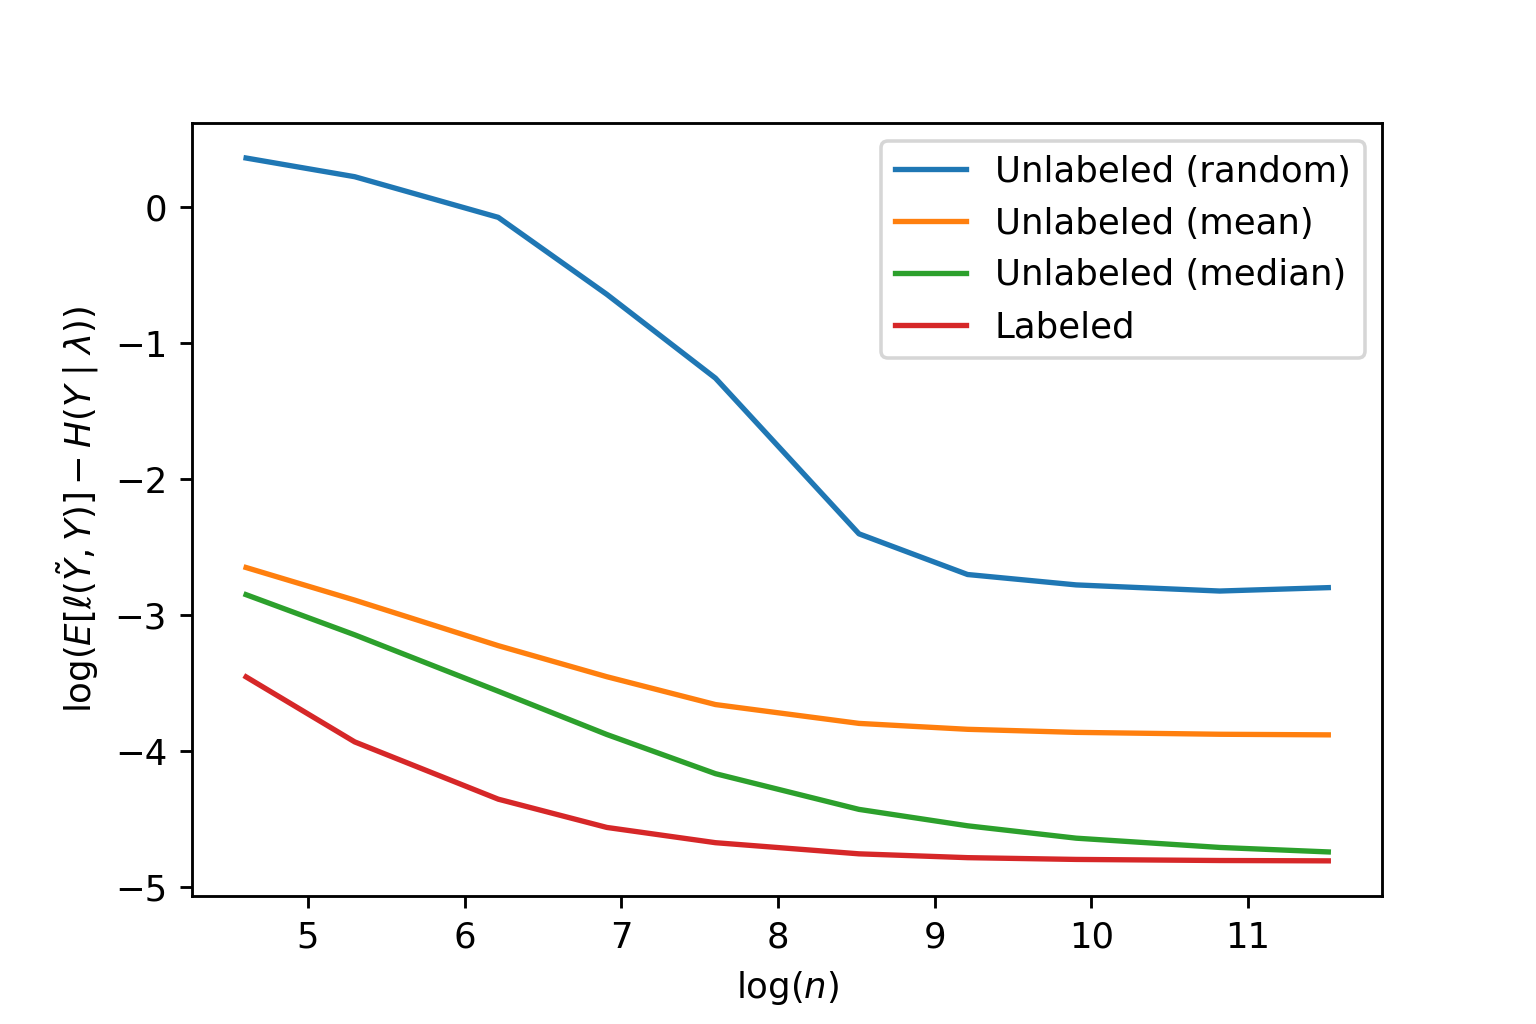
\includegraphics[width=.4\textwidth]{figures/misspecified_vary_n.png}
    %
    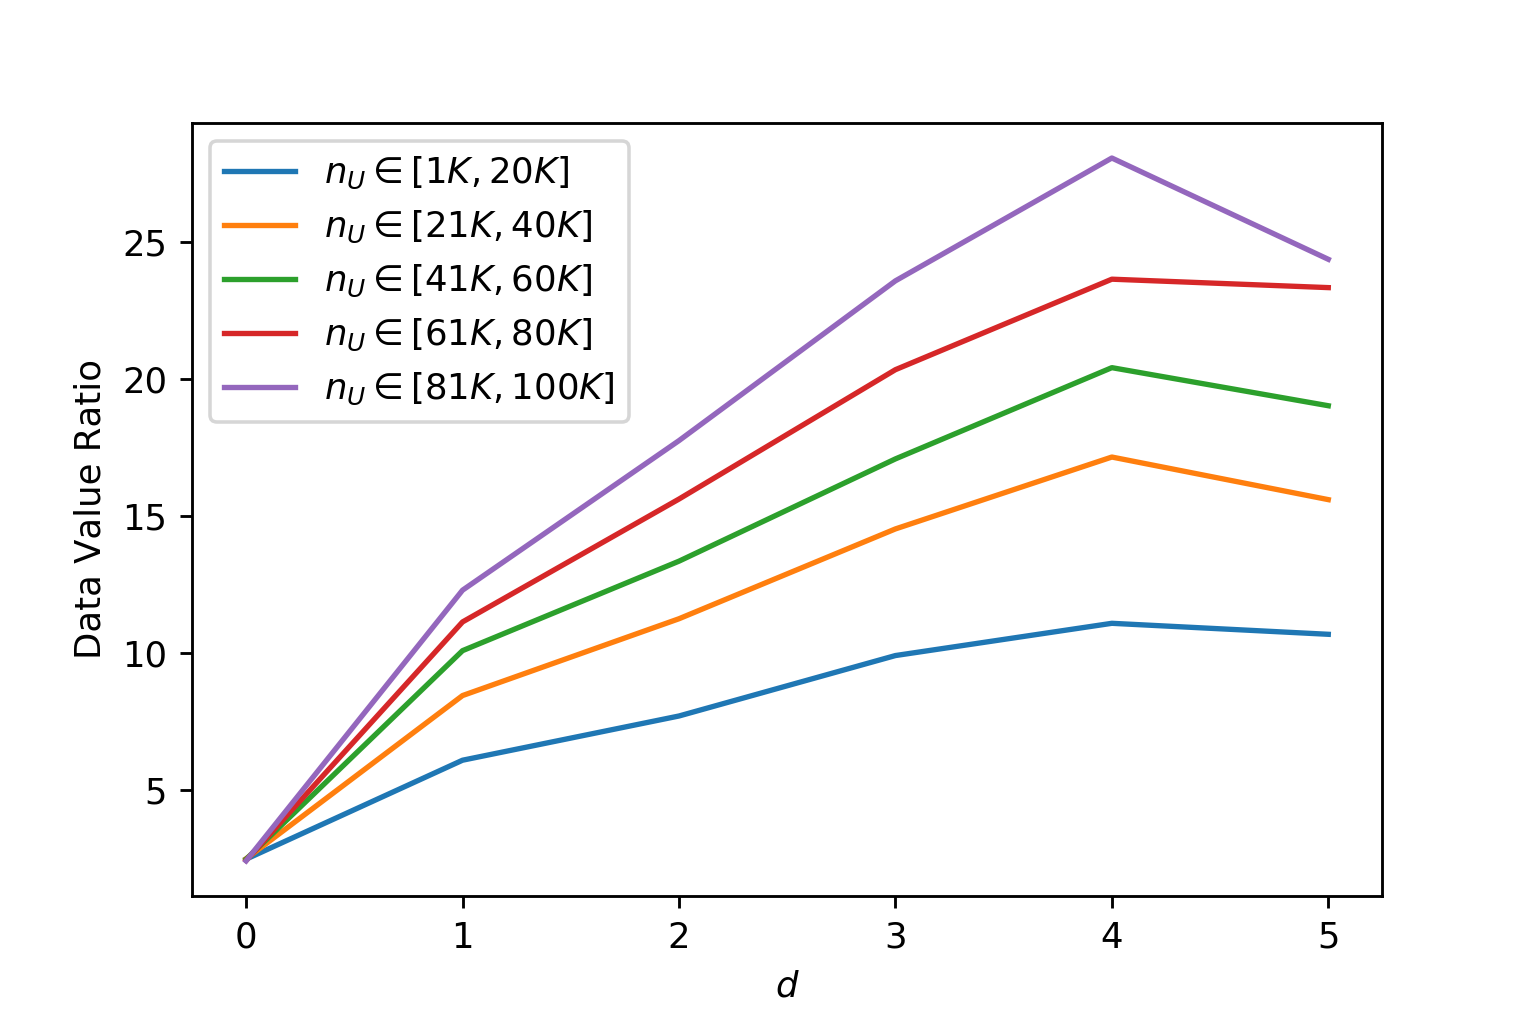
\includegraphics[width=.4\textwidth]{figures/data_value_ratio.png}
    \caption{Top: Log generalization error vs. $\log(n)$ with different estimators for synthetic data with $d=5$. We see that learning from unlabeled data results in a standing bias due to misspecification, and that median aggregation corrects for this bias. Bottom: Data value ratio vs. $d$ for a corrected estimator. We see that in the well-specified case ($d=0$) the data value ratio is small and roughly constant across $n$, and that the data value ratio grows with $d$, confirming that labeled data becomes more valuable with more misspecification.}
    \label{fig:ldvr_property}
\end{figure}

\paragraph{Protocol}

Our synthetic data distributions have balanced classes (i.e., $\mathbb{E}[Y]=0$) and $m=12$ labeling functions, with accuracies drawn uniformly from $[0.55, 0.75]$. Dependency strengths are fixed at $\varepsilon_{ij}=0.1$. To measure the expected generalization error of some learning algorithm, we perform $1000$ trials and average results, drawing data independently for each trial.

\paragraph{Results}

{\color{red} Combination table goes here. Shows four columns: all labeled, all unlabeled, naive combination, and James-Stein.}


\subsection{Value of Data on Real-World Datasets}
Next, we validate our findings in real-world datasets. In this case, we do not a priori know the level of misspecification. We expect that LFs are neither completely conditionally independent nor so markedly (conditionally) dependent that nothing can be learned from unlabeled data. This leads to data value ratios that are in between the scenarios in between the two extreme synthetic cases we considered above.

\begin{table}[t]
\caption{F1-scores for weakly labeled, labeled and hybrid approaches over the \textbf{Spam} and \textbf{Spouse} datasets.}
\label{sample-table}
\vskip 0.15in
\renewcommand{\arraystretch}{1.25} % Default value: 1
\begin{center}
\begin{small}
\begin{tabular}{lcccccr}
\hline
\textbf{Task} & $n_U$ & $n_L$ & \bfseries{\scshape{FlyingSquid}} & \bfseries{\scshape{MLE}} & \bfseries{\scshape{Hybrid}} \\
\hline
Spam    & 1586 & 40 & 82.35 & 82.40 & 83.16 \\
Spouse  & 3858 & 100 & 19.30 & 23.12 & 27.42 \\
\hline
\end{tabular}
\end{small}
\end{center}
\vskip -0.1in
\end{table}

\begin{figure}
    \centering
    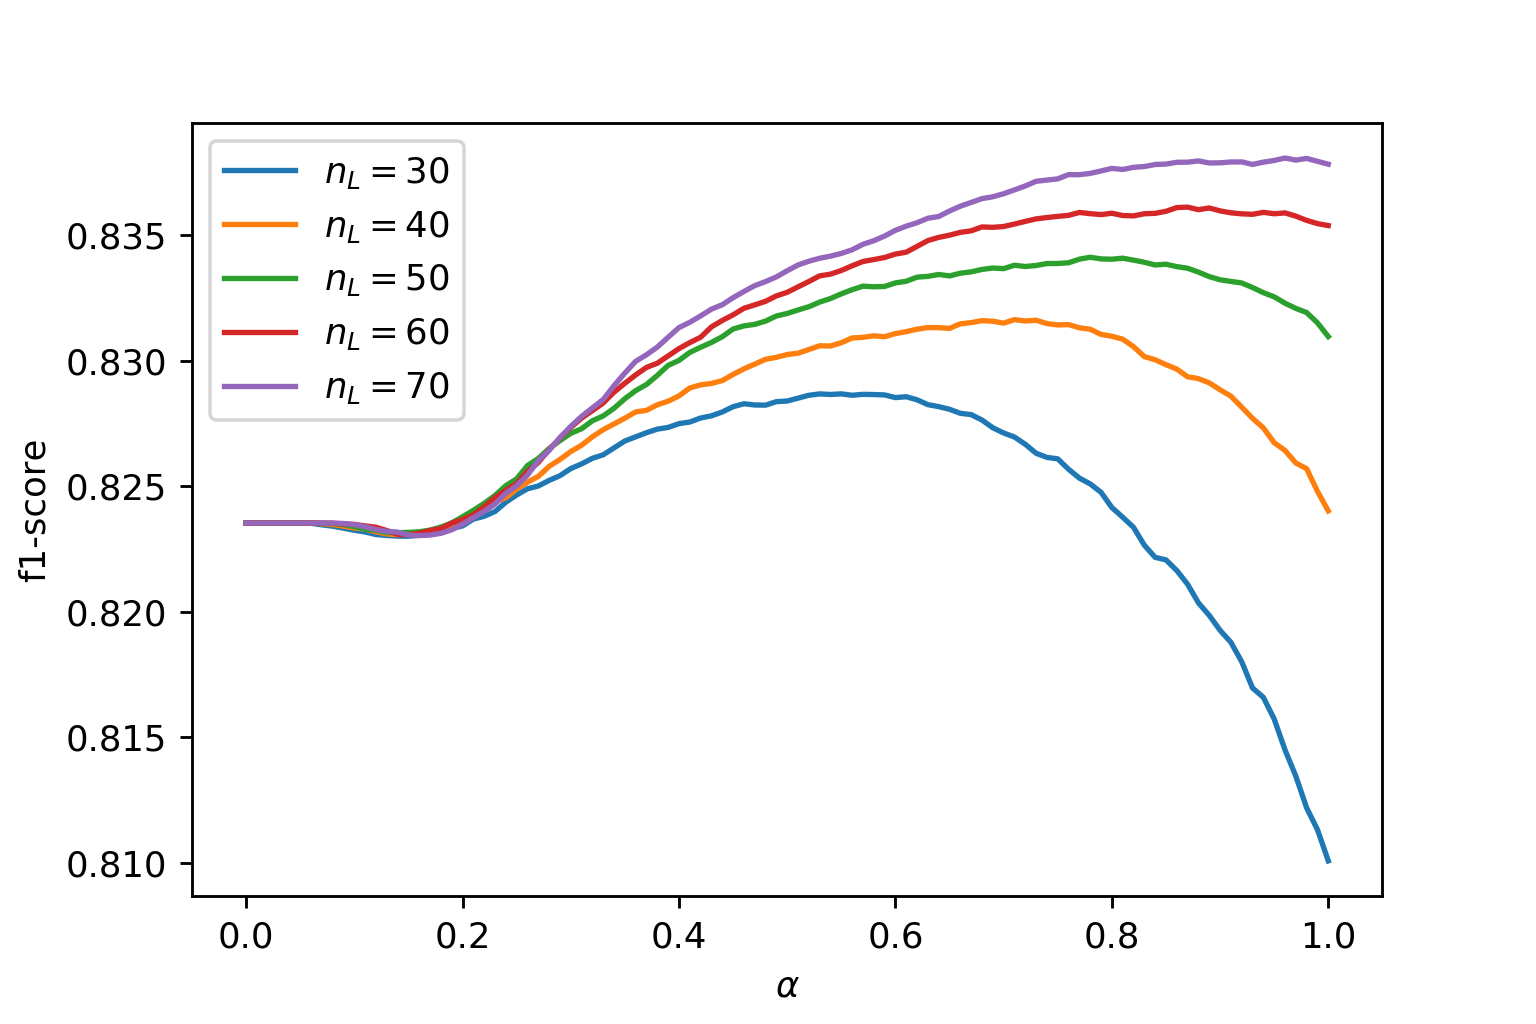
\includegraphics[width=.48\textwidth]{figures/spam_combined_estimator.png}
    \caption{F1-score of a combined estimator varying combination weight $\alpha$ on the \textbf{Spam} dataset for different labeled budgets $n_L$ (the weakly labeled budget is the entire dataset). We see that combining labeled and weakly labeled approaches can outperform either individually.}
    \label{fig:spam_combined_estimator}
\end{figure}

\paragraph{Protocol}
We use two tasks. First, \textbf{Spam} classification for Youtube comments  \cite{alberto2015tubespam} has $10$ LFs from \cite{Ratner19}. Here, the training set has $1586$ examples and the test set has $250$ examples; classes are approximately balanced. 

For each dataset we train models with different label budgets $n_L$. We report the average accuracy on the test set over $1000$ trials (with different points to label selected for each trial). 

\paragraph{Results}

\subsection{Weak Labels, Standing Bias, and Downstream Models}
Next, we measure the impact of bias in weak labels on end models trained on weak labels. We expect that when the weak labels do not have a standing bias, the generalization error is asymptotically identical to the case of training on fully-supervised labels. On the other hand, we hypothesize that biased weak labels will be reflected with a biased downstream model, no matter how much data we use, and that this bias is also a function of misspecification. That is, we expect that downstream models may not always be robust to weak labels.

\paragraph{Protocol}
{\color{red} Gathering models for this step.}

\paragraph{Results}
{\color{red} todo}

% \begin{figure}
%     \centering
%     \begin{minipage}{0.49\textwidth}
%         \centering
%         \includegraphics[width=0.9\textwidth]{figures/spam.pdf}
%         \caption{Accuracy for the \textbf{Spam} dataset with different budgets of labels and different unlabeled data weights $\gamma$.}
%         \label{fig:spam}
%     \end{minipage}\hfill
%     \begin{minipage}{0.49\textwidth}
%         \centering
%         \includegraphics[width=0.9\textwidth]{figures/amazon_reviews_1000.pdf}
%         \caption{Accuracy for the \textbf{Amazon Reviews} dataset with different budgets of labels and different unlabeled weights $\gamma$.}
%         \label{fig:amazon_reviews}
%     \end{minipage}
% \end{figure}
